
\paragraph{GET /:lang/user/:userId/question}
\begin{itemize}
\item \textbf{Successo}
Questo scenario rappresenta la richiesta che ritorna tutte le domande create da un utente.

\begin{figure}[ht]
	\centering
	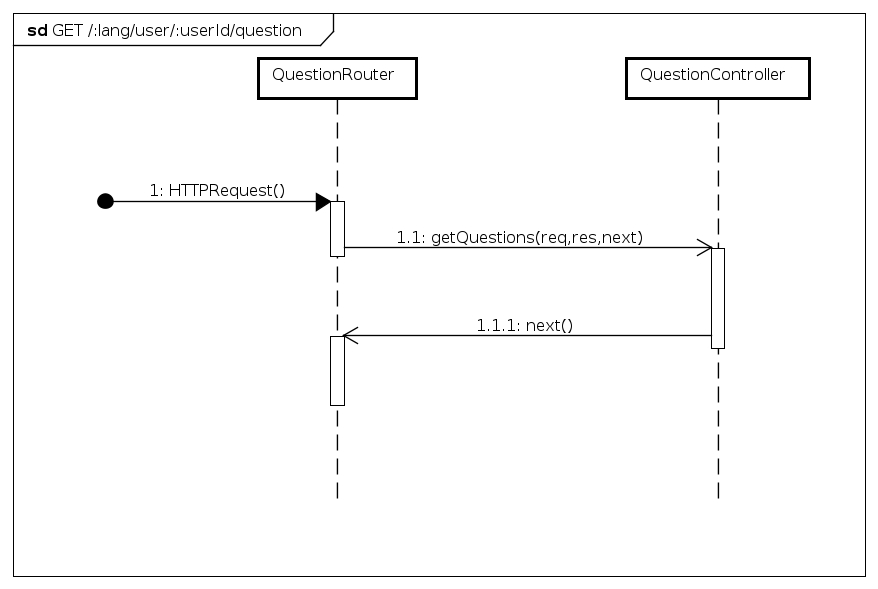
\includegraphics[scale=0.45]{UML/DiagrammiDiSequenza/Back-end/GET__lang_user__userId_question_success.png}
	\caption{Successo: GET /:lang/user/:userId/question}
\end{figure}
\FloatBarrier

\item \textbf{Fallimento}
Questo scenario rappresenta la richiesta che ritorna tutte le domande create da un utente non andata a buon fine; in questo caso il modulo \texttt{QuestionController} ritornerà un \texttt{next(err)} al router che avrà il compito di reinstradarlo (indirizzandolo verso \texttt{ErrorHandler}).

\begin{figure}[ht]
	\centering
	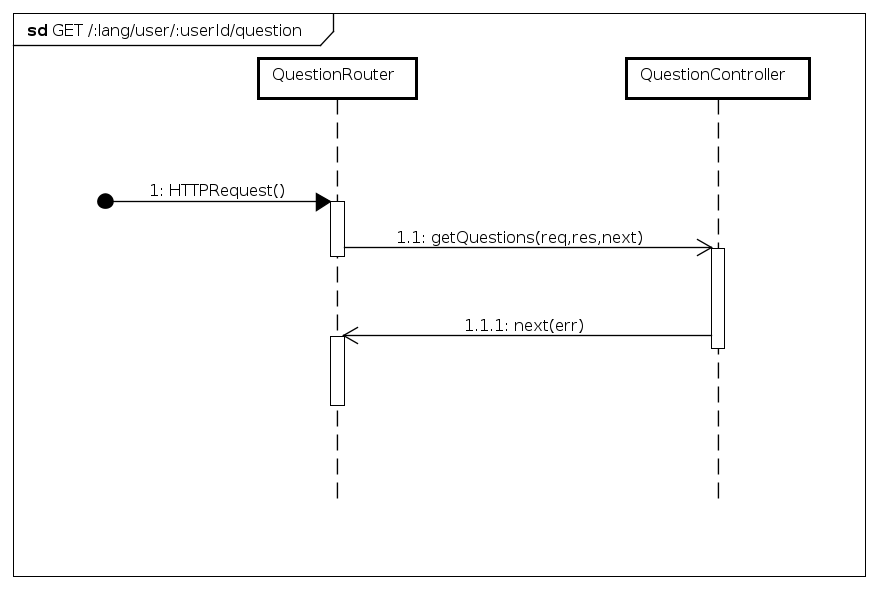
\includegraphics[scale=0.45]{UML/DiagrammiDiSequenza/Back-end/GET__lang_user__userId_question_failure.png}
	\caption{Fallimento: GET /:lang/user/:userId/question}
\end{figure}
\FloatBarrier

\end{itemize}






\paragraph{GET /:lang/user/:userId/question/:questionId}
\begin{itemize}
\item \textbf{Successo}


\begin{figure}[ht]
	\centering
%	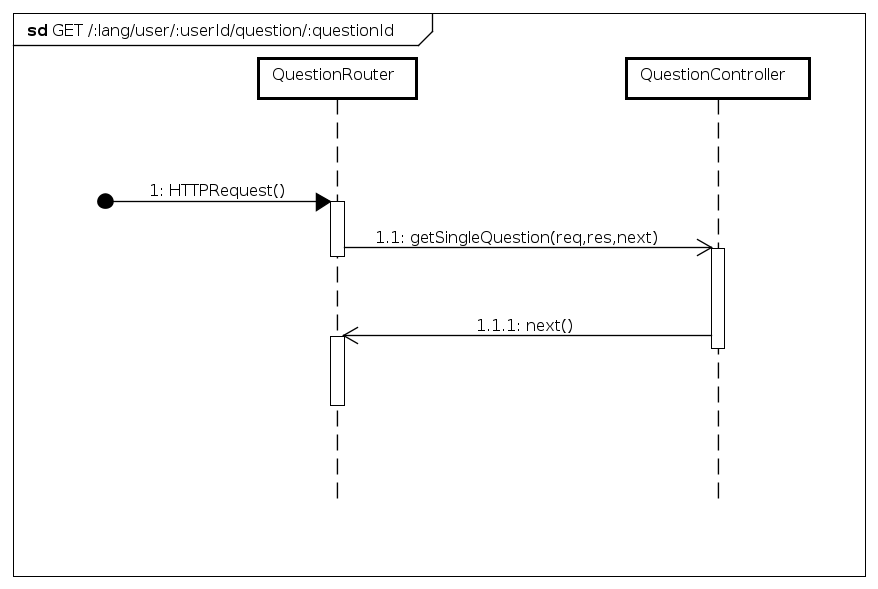
\includegraphics[scale=0.45]{UML/DiagrammiDiSequenza/Back-end/GET__lang_user__userId_question__questionId_success.png}
	\caption{Successo: GET /:lang/user/:userId/question}
\end{figure}
\FloatBarrier

\item \textbf{Fallimento}


\begin{figure}[ht]
	\centering
	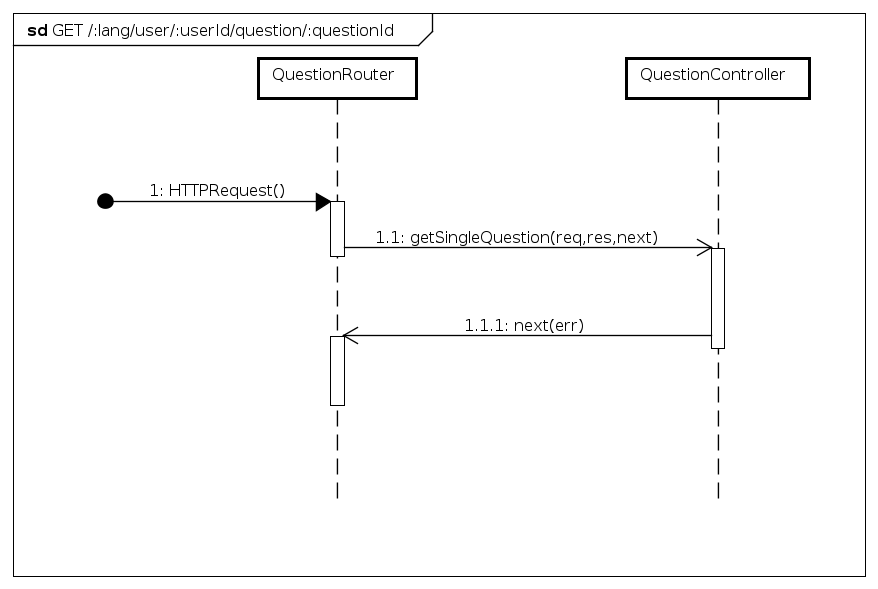
\includegraphics[scale=0.45]{UML/DiagrammiDiSequenza/Back-end/GET__lang_user__userId_question__questionId_failure.png}
	\caption{Fallimento: GET /:lang/user/:userId/question}
\end{figure}
\FloatBarrier

\end{itemize}






\paragraph{POST /:lang/user/:userId/question}
\begin{itemize}
\item \textbf{Successo}
Questo scenario rappresenta la richiesta che inserisce una nuova domanda creata da un utente all'interno del sistema.


\begin{figure}[ht]
	\centering
	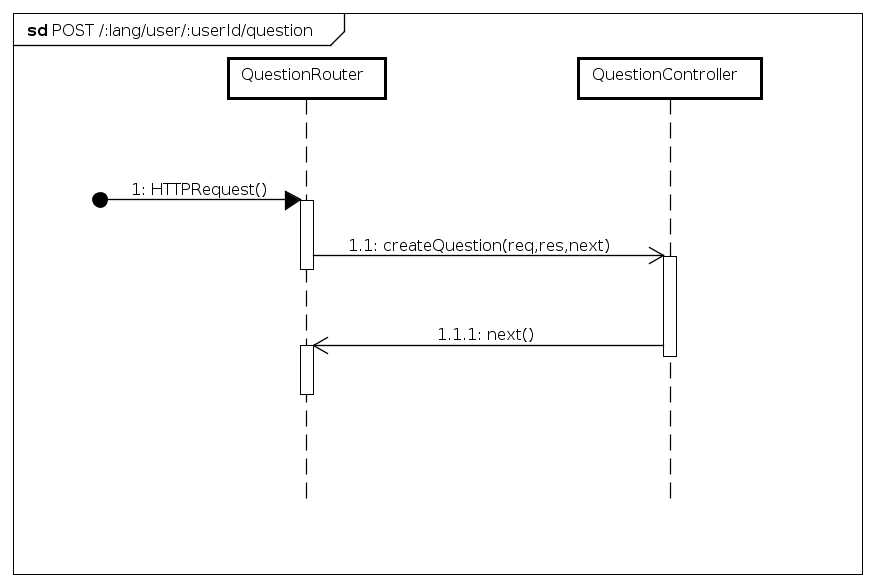
\includegraphics[scale=0.45]{UML/DiagrammiDiSequenza/Back-end/POST__lang_user_question_success.png}
	\caption{Successo: POST /:lang/user/:userId/question}
\end{figure}
\FloatBarrier

\item \textbf{Fallimento}
Questo scenario rappresenta la richiesta che inserisce una nuova domanda creata da un utente all'interno del sistema non andata a buon fine; in questo caso il modulo \texttt{QuestionController} ritornerà un \texttt{next(err)} al router che avrà il compito di reinstradarlo (indirizzandolo verso \texttt{ErrorHandler}).

\begin{figure}[ht]
	\centering
	\includegraphics[scale=0.45]{UML/DiagrammiDiSequenza/Back-end/POST__lang_user_question_failure.png}
	\caption{Fallimento: POST /:lang/user/:userId/question}
\end{figure}
\FloatBarrier

\end{itemize}
